\begin{frame}\label{a.3}
\frametitle{Elastic Dynamical Facilitation (EDF) Theory: The Complete Picture}

EDF theory unifies elasticity with glassy dynamics through \textbf{three interconnected pillars} that provide a complete microscopic framework:

\vspace{0.5em}

\begin{columns}[T]
\begin{column}[T]{0.33\textwidth}

\centering\textbf{\Large Excitations}

\begin{figure}[t]
\centering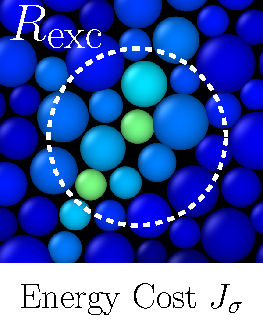
\includegraphics[height=0.45\textheight]{a.2-intro_dftheory/DF_Theory_Excitations_Zoom_2.pdf}
\caption{\textbf{Pure shear excitations} with energy scale $J_\sigma \sim G R_\mathrm{exc}^2 \epsilon_\mathrm{c}^2$}
\end{figure}

\end{column}

\begin{column}[T]{0.33\textwidth}

\centering\textbf{\Large Onset Temperature}

\begin{figure}[t]
\begin{center}
\centerline{\includegraphics[height=0.45\textheight]{c.1-kt_msdintro/msd-supercooledliq-5.pdf}}
\end{center}
\caption{\textbf{2D melting theory} explains $T_\mathrm{o}$ from elastic stability}
\end{figure}

\end{column}

\begin{column}[T]{0.33\textwidth}

\centering\textbf{\Large Facilitation}

\begin{figure}[t]
\begin{center}
\centerline{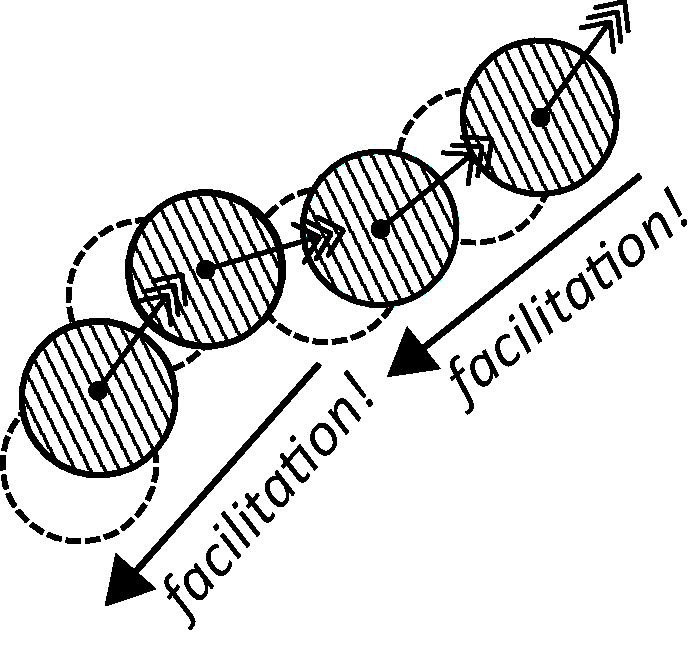
\includegraphics[height=0.45\textheight]{a.2-intro_dftheory/facilitation_closer_2.pdf}}
\end{center}
\caption{\textbf{Elastic stress fields} create emergent facilitation}
\end{figure}

\end{column}
\end{columns}

\vspace{1em}

\begin{block}{\centering Key Insight}
\centering \textbf{Elasticity} provides the microscopic foundation for all three pillars, creating a \textbf{unified quantitative theory}: 
$$\boxed{\text{EDF Theory} = \text{Elastic Excitations} + \text{Elastic Onset} + \text{Elastic Facilitation}}$$
\end{block}

\end{frame} 